\chapter{Introduction}

Quasar, short for "quasi-stellar radio source", also known as "QSO" (quasi-stellar object), is one of nature's wonders. They are some very distant objects with extremely high luminosity. In fact, quasars are a type of active galactic nuclei (AGNs). The word 'quasar' was first introduced by \citet{chiuGravitationalCollapse1964} to stand for a kind of point source with strong radio emissions. With more and more observations taken, researchers began to realize not all 'quasars' have strong radio transmission. Actually, \citet{kellermannVLAObservationsObjects1989,ivezicOpticalRadioProperties2002} estimated that only about $10\%$ of this type objects are actually "radio-loud". Consequently, the term "QSO" (Quasi-Stellar Object) was adopted as a more inclusive designation, while "quasar" remains the widely used for both radio-loud and radio-quiet objects in general writing \citep{shieldsBriefHistoryActive1999}. 

As the name suggets, quasars are faint and point-like objects somewhat like distant stars. 

\section{History of Quasars}

Researchers began to have a glimpse to quasars in the late 1950s with the development of early radio astronomy. A series of Large-scale radio surveys, such as the Third Cambridge Catalogue of Radio Sources (3C) \citep{edgeSurveyRadioSources1959, bennettPreparationRevised3C1962}, identified many powerful radio emitters without counterparts in optical band. Through optical telescopes, these targets appeared point-like (similar to stars) rather than extended sources like galaxies.

The important breakthrough occurred in 1963 when astronomer Maarten Schmidt examined the optical spectrum of the radio source 3C 273 taken by the 200-inch (5.1 m) Hale Telescope on Mount Palomar. Schmidt realized that the unresolvable emission lines in its spectrum were not from unknown elements, but were just simply ordinary hydrogen lines with an unprecedented redshift $z = 0.158$‬‬ \citep{schmidt3C273StarLike1963}. This massive redshift implied that 3C 273 was an exceedingly distant object. Therefore, it must be radiating energy at an incredible scale that couldn't be explained by contemporary physics.

As the finding of the quasar with high redshift ($z > 0.1$), scientists could begin to have a look at high-redshift universe. Quasars became almost the only way for astronomers to research early universe and cosmological evolution before the instrument could detect such distant galaxies. 

At the same time, throughout the late 1960s and 1970s, the theoretical framework was also developing rapidly. Astrophysicists, notably \citet{lynden-bellGalacticNucleiCollapsed1969}, based on \citet{salpeterAccretionInterstellarMatter1964},  proposed that the immense luminosity of quasars could only be possibly generated by mass accretion onto a supermassive black hole with gravity. This theorem established the foundational standard model for Active Galactic Nuclei (AGN) that remains central to astrophysics until today.

\section{Unified Model and Subtypes for Quasars}

At the core of a quasar, it is powered by a supermassive black hole at the centre of a distant galaxy, which is the host galaxy of this quasar. As surrounding gas and dust fall into the black hole's immense gravitational well, they form an accretion disk with very high energy. The extreme friction and gravitational forces heat this material, causing it to emit incredible huge amounts of radiation among the entire electromagnetic spectrum, frequently covering the combined light of all the stars in the host galaxy. Figure~\ref{fig:qso_model} illustrates the physical model of quasars.

Beyond the central accretion disk, the standard Unified Model also points out that this central engine is surrounded by a geometrically and optically thick structure of dust and gas, commonly referred to as the dusty torus \citep{antonucciUnifiedModelsActive1993}. Further out, clouds of gas orbit the black hole at different distances, forming the Broad-Line Region (BLR) with higher density close to the center and the less dense Narrow-Line Region (NLR) in higher distances area. According to the Unified Model, the vast observational diversity of quasars is primarily a geometric effect, dictated by the observer's viewing angle relative to this obscuring torus \citep{urryUnifiedSchemesRadioLoud1995}.

\begin{figure}[htbp]
    \centering
    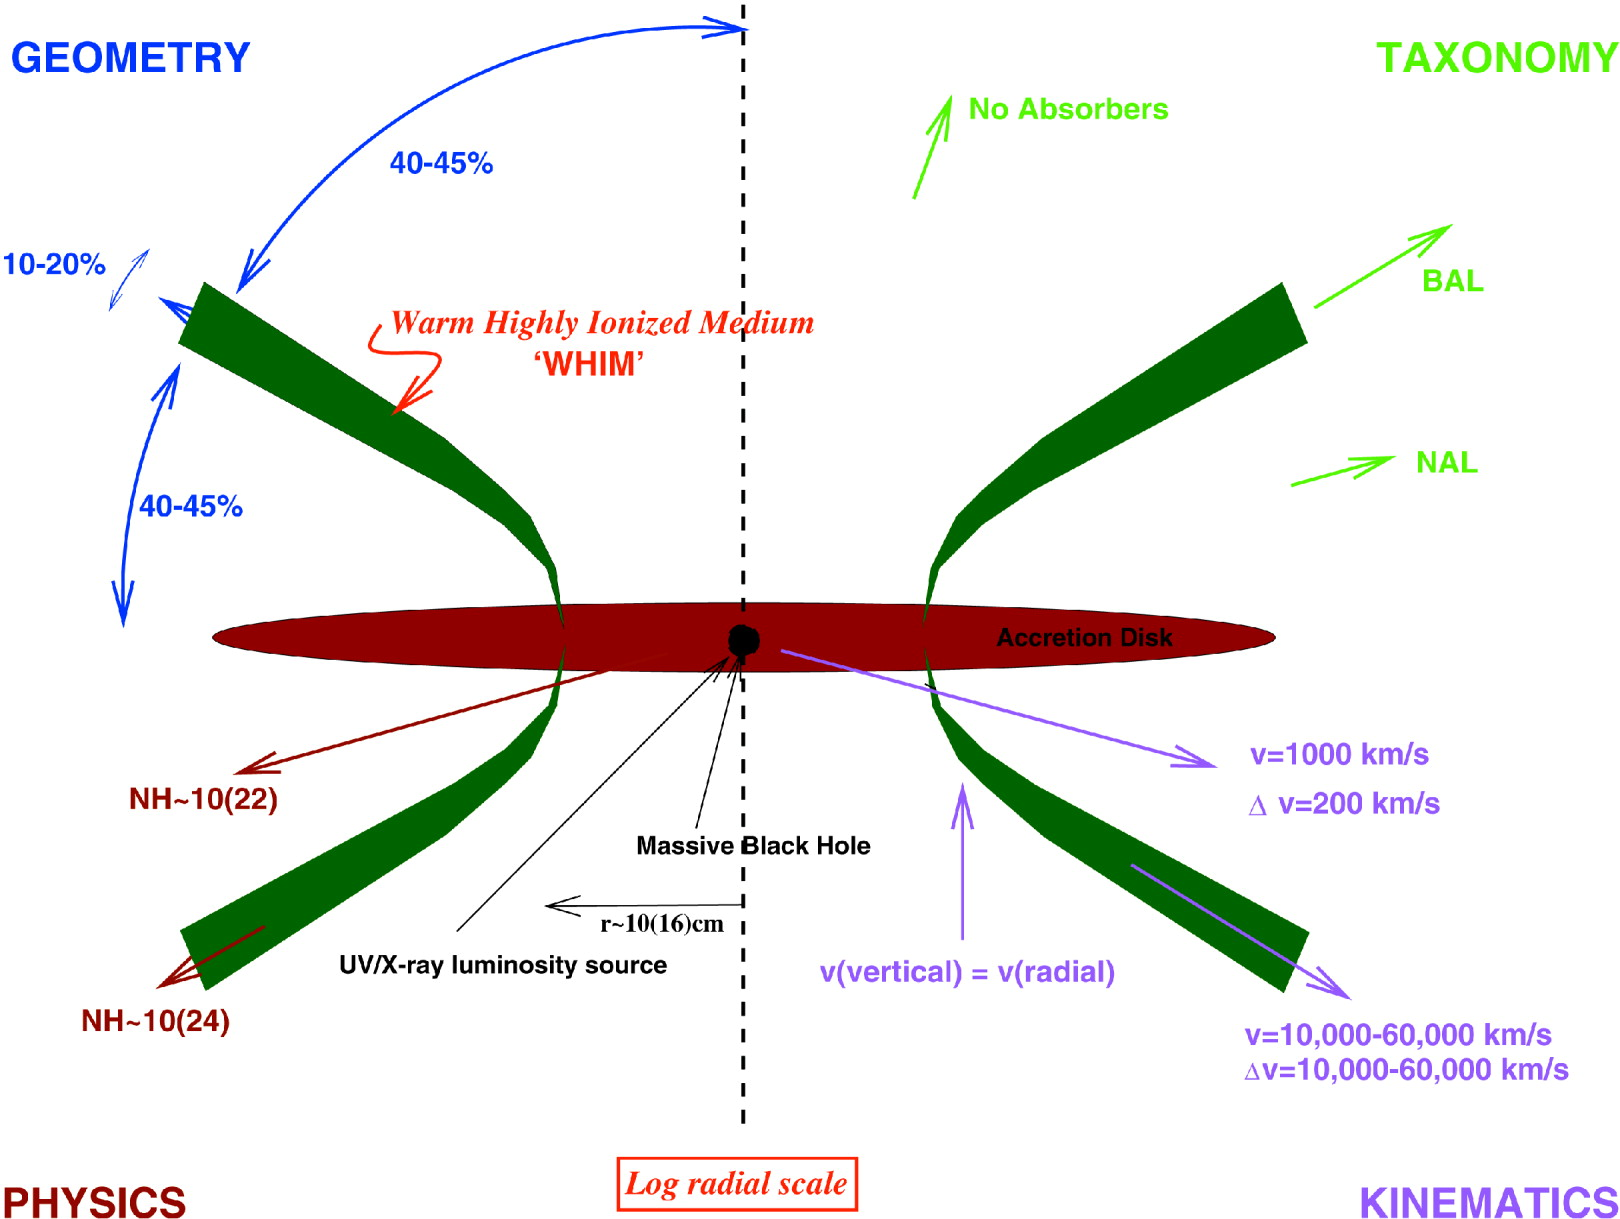
\includegraphics[width=1\linewidth]{paper//figs//intro/10_1086_317778_fg1_hr.jpg}
    \caption{Proposed structure. The four symmetric quadrants illustrate the following (clockwise from top left): the opening angles of the structure, the spectroscopic appearance to a distant observer at various angles, the outflow velocities along different lines of sight, and some representative radii (appropriate for the Seyfert 1 galaxy NGC 5548) and some typical column densities. \citep{elvisStructureQuasars2000}}
    \label{fig:qso_model}
\end{figure}

Based on this orientation, quasars can be classified into two main optical subtypes:
\begin{itemize}
\item \textbf{Type 1 Quasars:} These are viewed nearly pole to us. Because our line of sight does not pass through the dusty torus, we can observe directly into the innermost regions. Consequently, their optical spectra display both strong continuum emission from the accretion disk and highly broadened emission lines (with velocities of thousands of kilometres per second) originating from the fast-moving gas in the BLR.

\item \textbf{Type 2 Quasars:} These are viewed nearly edge-on. The dense dusty torus cuts the direct view to the accretion disk and the BLR. Therefore, their optical spectra don't have broad emission lines and are instead by narrow emission lines, which originate from the slower-moving, unobscured gas in the extended NLR \citep{netzerRevisitingUnifiedModel2015}.
\end{itemize}
In Figure~\ref{fig:qso_class}, it shows the connection between subtypes to the unified model of AGNs.

Additionally, while most of quasars are "radio-quiet", the "radio-loud" objects have powerful, collimated relativistic jets of plasma extending perpendicular to the accretion disk. In the extreme scenario where one of these jets points directly along our line of sight, the radiation is relativistically beamed and significantly amplified. Such objects are classified as \textbf{blazars} (comprising to BL-Lacertae objects and Flat-Spectrum Radio Quasars), characterized with rapid variability and strong polarization \citep{blandfordRelativisticJetsCompact1979}.

\begin{figure}[htbp]
    \centering
    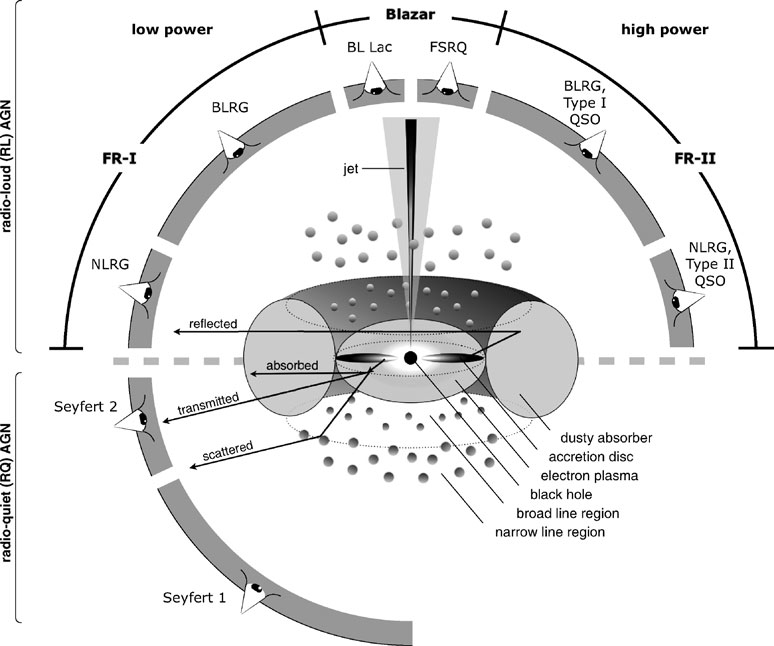
\includegraphics[width=1\linewidth]{paper//figs//intro/class.png}
    \caption{Schematic representation of our understanding of the AGN phenomenon in the unified scheme. The type of object we see depends on the viewing angle, whether or not the AGN produces a significant jet emission, and how powerful the central engine is. Note that radio-loud objects are generally thought to display symmetric jet emission. Graphic by Marie-Luise Menzel. \citep{beckmannActiveGalacticNuclei2012}}
    \label{fig:qso_class}
\end{figure}

\begin{figure}[htbp]
    \centering
    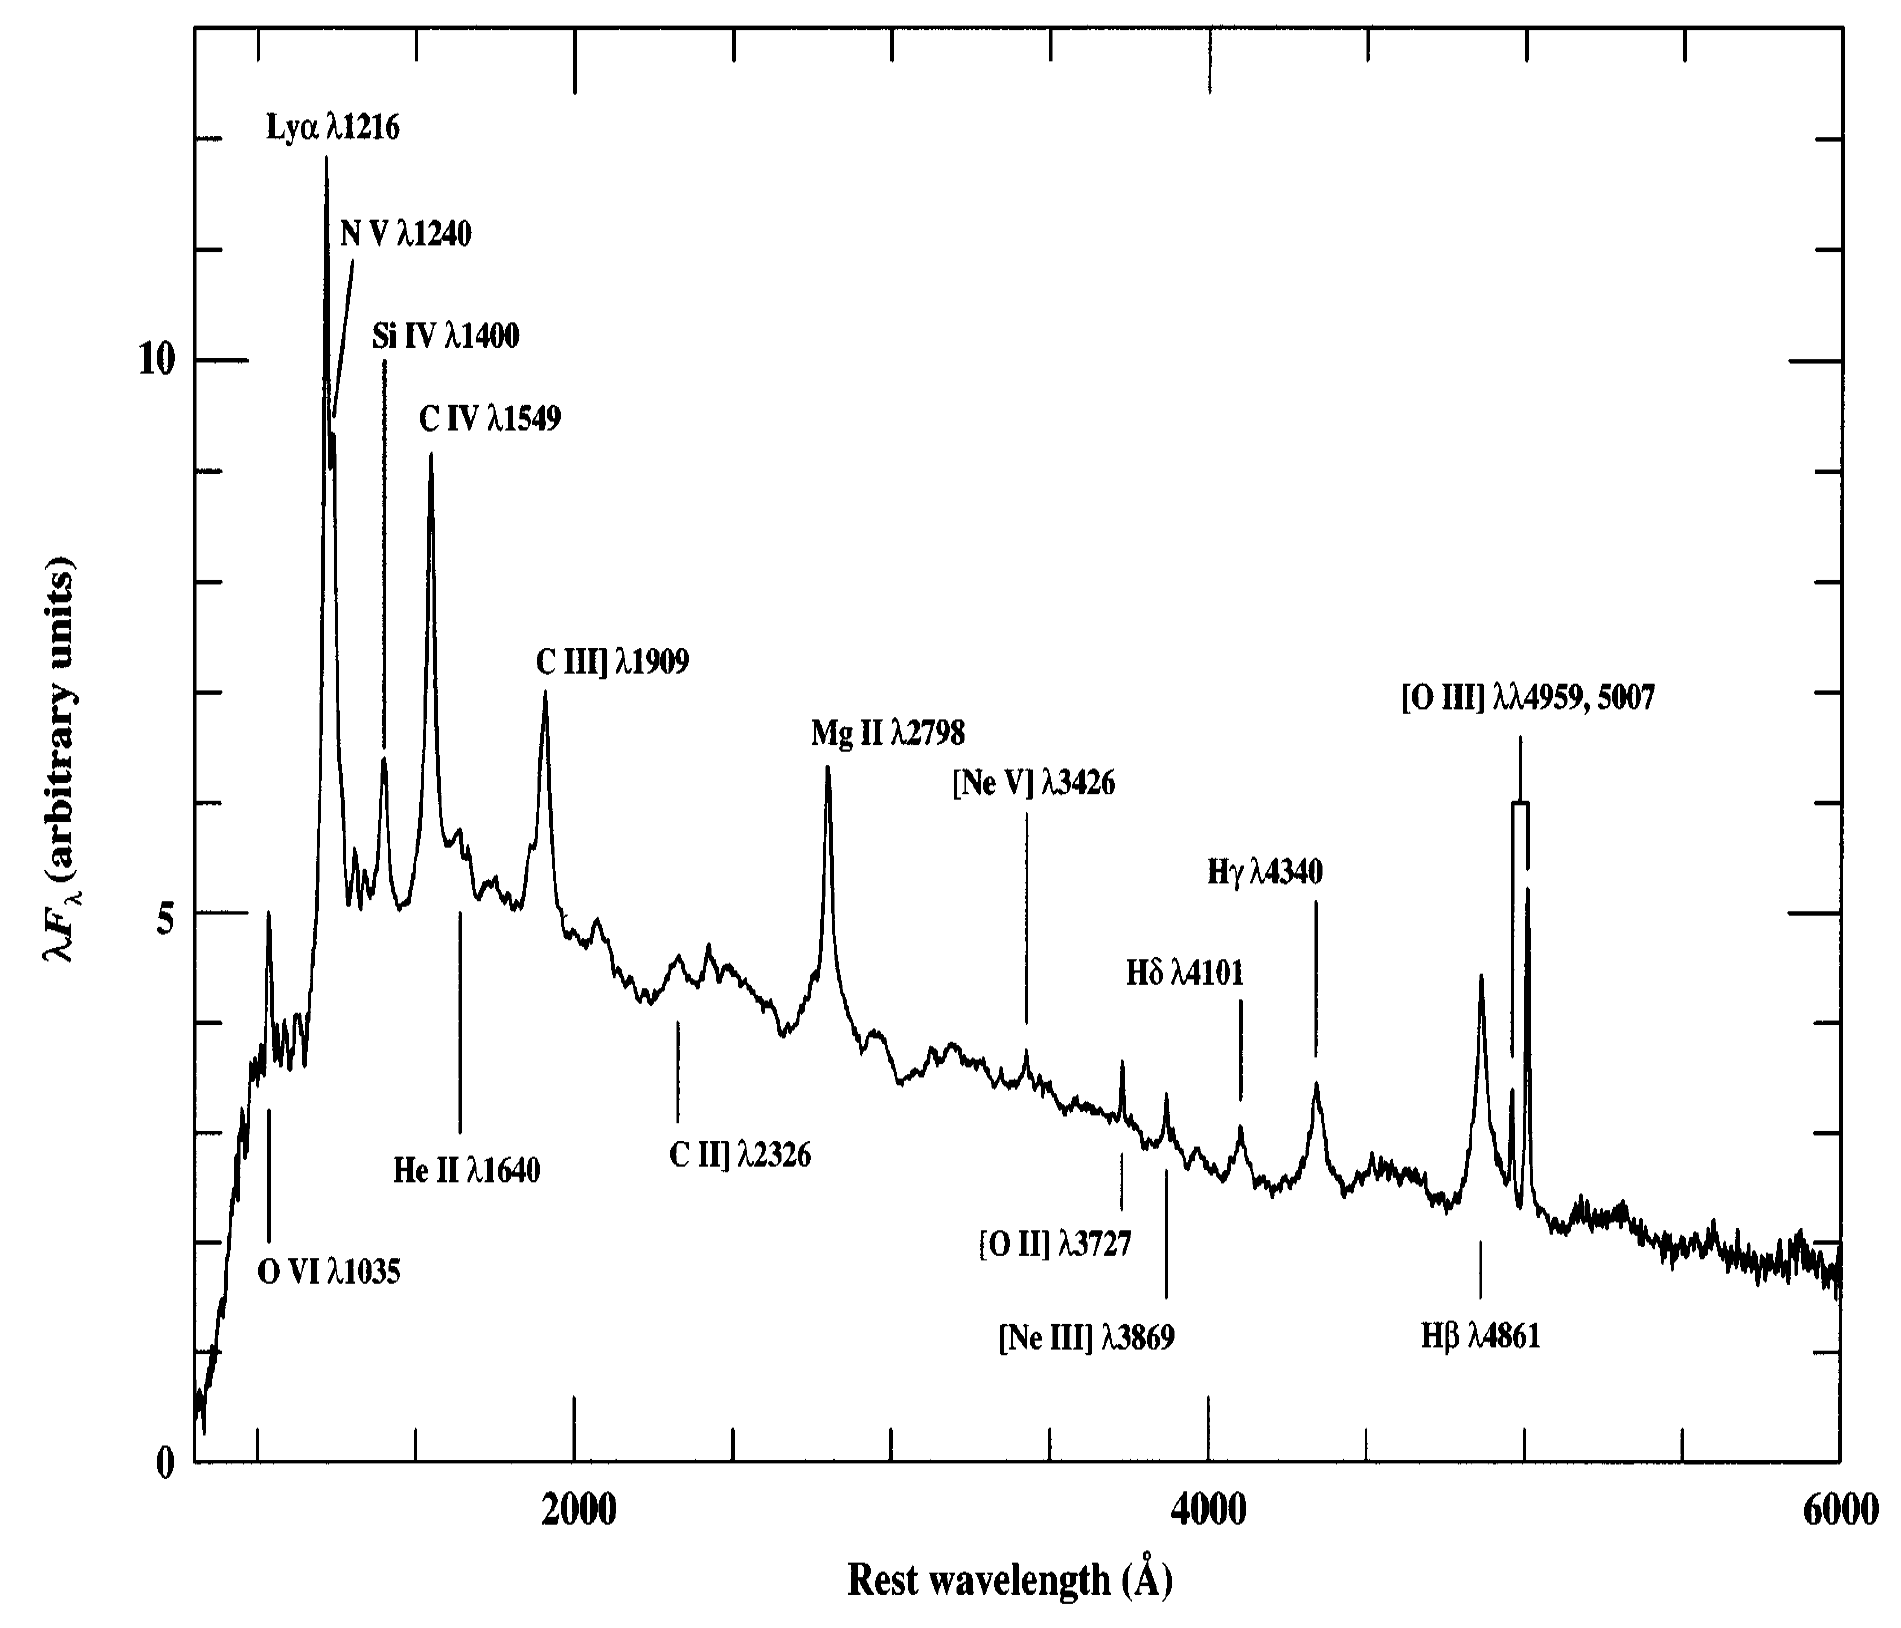
\includegraphics[width=1\linewidth,height=0.45\textheight]{paper//figs//intro/spec-temp.png}
    \caption{A mean QSO spectrum formed by averaging spectra of over 700 QSOs from the Large Bright Quasar Survey \citep{francisHighSignaltonoiseRatio1991}. Prominent emission lines are indicated. \citep{peterson_introduction_1997}}
    \label{fig:qso_model}
\end{figure}

\section{Selection Effects in Quasars}

When studying the distribution of quasars across the universe, astronomers must carefully account for observational biases known as selection effects. Because quasars are objects under extreme condition, astronomical catalogues do not represent the true underlying population, but rather a filtered subset dictated by instrumental limitations and survey designs.

There are some selection effects:

\paragraph{Radio-Loud and Radio-Quiet Bias} Early quasar discoveries relied heavily on radio surveys, which made the first generation quasar samples only contained radio-loud objects. As \citet{kellermannVLAObservationsObjects1989,ivezicOpticalRadioProperties2002} estimation, only $\sim10\%$ quasars have strong emission in radio band. Fortunately, as the improvement of detector sensitivity and development in multi-band astronomy, the effect of this bias has a sharp decrease nowadays.

\paragraph{Colour Selection Bias} Modern massive optical surveys, such as the Sloan Digital Sky Survey (SDSS), traditionally identify quasar candidates based on their distinct non-stellar colour features across broad photometric bands (e.g., $u, g, r, i, z$‬) \citep{richardsSpectroscopicTargetSelection2002}. However, a bias arises at specific redshifts, particularly around $z \approx 2.7$‬‬. At this epoch, the strong Lyman-$\alpha$‬ ($\text{Ly}\alpha$‬) emission line and the closed Lyman limit shift directly into the optical $g$‬ and $r$‬ passbands. Consequently, the distinct power-law signature of a quasar is deeply changed, causing its broad-band optical colours (such as $u-g$‬‬ and $g-r$‬‬) to perfectly cover the thermal spectra of main-sequence A-type and F-type stars in usual optical colour-colour diagrams. This degeneracy causes a significant decrease in detection efficiency, creating an artificial "redshift gap" as incompleteness in the observed distribution of quasars.

To reduce this optical colour selection bias, modern astronomy relies on multi-wavelength observations more. For instance, if we move into the near-infrared, surveys base on the $K$‬-band excess (KX) method \citep{maddoxLargeAreaKX2012}, which contrasts the red power-law continuum of quasars against the rapidly declining Rayleigh-Jeans tail of stellar blackbody emission. Furthermore, the Wide-field Infrared Survey Explorer (WISE) made mid-infrared selections with high efficiency. The heated dust in the AGN torus produces an obvious mid-infrared excess that easily classifies quasars from stars just using simple colour thresholds ($W1 - W2 \ge 0.8$‬‬), virtually avoid the $z \approx 2.7$‬ optical bottleneck and recovering heavily dust-obscured populations \citep{2012ApJ...753...30S,2013ApJ...772...26A}. We can also find this in the survey result shown in Chapter~\ref{chpt:res}.

Also, To check and try to fully avoid the bias from colour selection, \citet{krogager_4mostgaia_2023} introduced Purely Astrometric Quasar Survey (PAQS), which is only based on purely astrometric selection method to find quasar candidates. This method is introduced by \citet{heintz_study_2015} and had an initial verification in \citet{heintz_spectroscopic_2020}. We will describe this method with more detail in Chapter \ref{sec:selection}.

\section{Introduction of SNAQS}

The Smaller  NOT  Astrometric  Quasar  Survey  (SNAQS) is a stepping stone survey for PAQS. With SNAQS we are pointing to build a $100\%$ complete sample of all quasars brighter than 19 Magnitude ($m_G<19$) in an area of 245 square degrees around the north galactic pole. This sample contains 1627 targets selected by purely astrometric selection method.

With this sample we aim to do:
\begin{itemize}
    \item Make the first statistical inquiries about $m_G<19$ quasars from a complete sample. 
    \item Measure the distributions of redshift and dust extinction.
    \item Measure the fraction of Broad Absorption Line quasars (BAL quasars).
    \item Characterize the most important contaminants (sources that are not quasars).
    \item Test and improve our classification and analysis software to be used in PAQS.
\end{itemize}

Also we can make a prediction for the result of PAQS by SNAQS. 

In Chapter~\ref{sec:selection}, we will discuss about the selection of observation targets for SNAQS. Then, in Chapter \ref{chpt:spec}, we will describe the data reduction and spectra analysis pipeline.

There will be a summary of SNAQS observation result in Chapter~\ref{chpt:res}, and talk about the finding from them in Chapter~\ref{chpt:dis}.
